\vspace{-15pt}
\section{System Design}\label{sec:design}
\vspace{-10pt}
We focus on the protection of the runtime stack under the following assumptions: (i) Flash memory and registers are not affected by SEUs. (ii) Only one SEU will occur during a given function execution. It is rare for more than one bit to be upset simultaneously; this occurs in only 5 to 6 percent of bit flip errors~\cite{underwood1992sramorbit}. 

Our approach is designed to align with the NASA coding standards for C applied in space projects~\cite{nasa_coding_standard}: First, dynamic memory allocation is not allowed, so the heap section in RAM is not used. However, for the sake of completeness, we consider the possibility of a non-empty heap in our approach. Second, the \texttt{goto} statement is not allowed. Finally, each function should have fewer than 60 lines of code, making the execution time of each function relatively short.

Our approach protects the system stack by introducing auxiliary assembly code. The new code is injected at both the beginning and end of each function or interrupt handler. When a function is called, the code injected at the beginning of the call calculates the CRC of the caller's stack frame and saves both the CRC and the stack frame. Before the callee returns, the code injected at the end calculates the CRC of the caller's stack frame again, compares it with the saved CRC, and restores the caller's stack frame if the CRCs do not match. 
\vspace{-15pt}
\subsection{Supporting Memory Sections}\label{sec:memory_sections}
\vspace{-5pt}
To store stack frame replicas, two new sections are created in SRAM just after the \texttt{.bss} section by modifying the linker script~\cite{linkerscript}. The new \texttt{md} section is used to store stack frame replicas, which are referred to as \textit{Stack Frame Snapshots} (SFSs). The new \texttt{sp} section is used to store the address of the next available memory space in \texttt{md}, similar to the stack pointer. This address is referred to as the \textit{Snapshot Top Pointer} (STP). To protect the STP from SEUs, the size of the \texttt{sp} section is set to 6 bytes, and 3 STP duplicates are stored in this section. Given that we assume only one SEU will occur during the execution of a given function, only one STP replica could be altered by a flipped bit. The altered STP is easily identified and corrected by comparing the values of the three STP replicas.
\vspace{-15pt}
\subsection{Injected Code Segments}
\vspace{-5pt}
The injected code segments are designed to use only registers, reducing their dependence on RAM. \textit{CRC Calculate} is used to calculate the CRC of a memory region. In our implementation, CRC16-CCITT is used~\cite{crc16}. \textit{CRC Save} is used to save the CRC to the stack. \textit{CRC Compare} is used to compare two CRCs. The comparison result indicates whether an SEU is detected. \textit{Frame Copy} is used to copy a stack frame to a given destination, and to save and restore stack frames. \textit{Frame Size Save} is used to save the size of the stack frame for the current function. \textit{STP Initialize} is used to initialize the STP so it points to the lowest address of the \texttt{md} section. \textit{STP Update} is used to update the STP. First, it obtains the correct STP value by comparing the three STP replicas. The replicas are then updated to reflect the addition or removal of a stack frame.
\vspace{-15pt}
\subsection{Modified Function Execution Process}
\vspace{-5pt}
\subsubsection{Modified Function Invocation Process.}
\vspace{-15pt}
\begin{figure}[h]
	\centering
	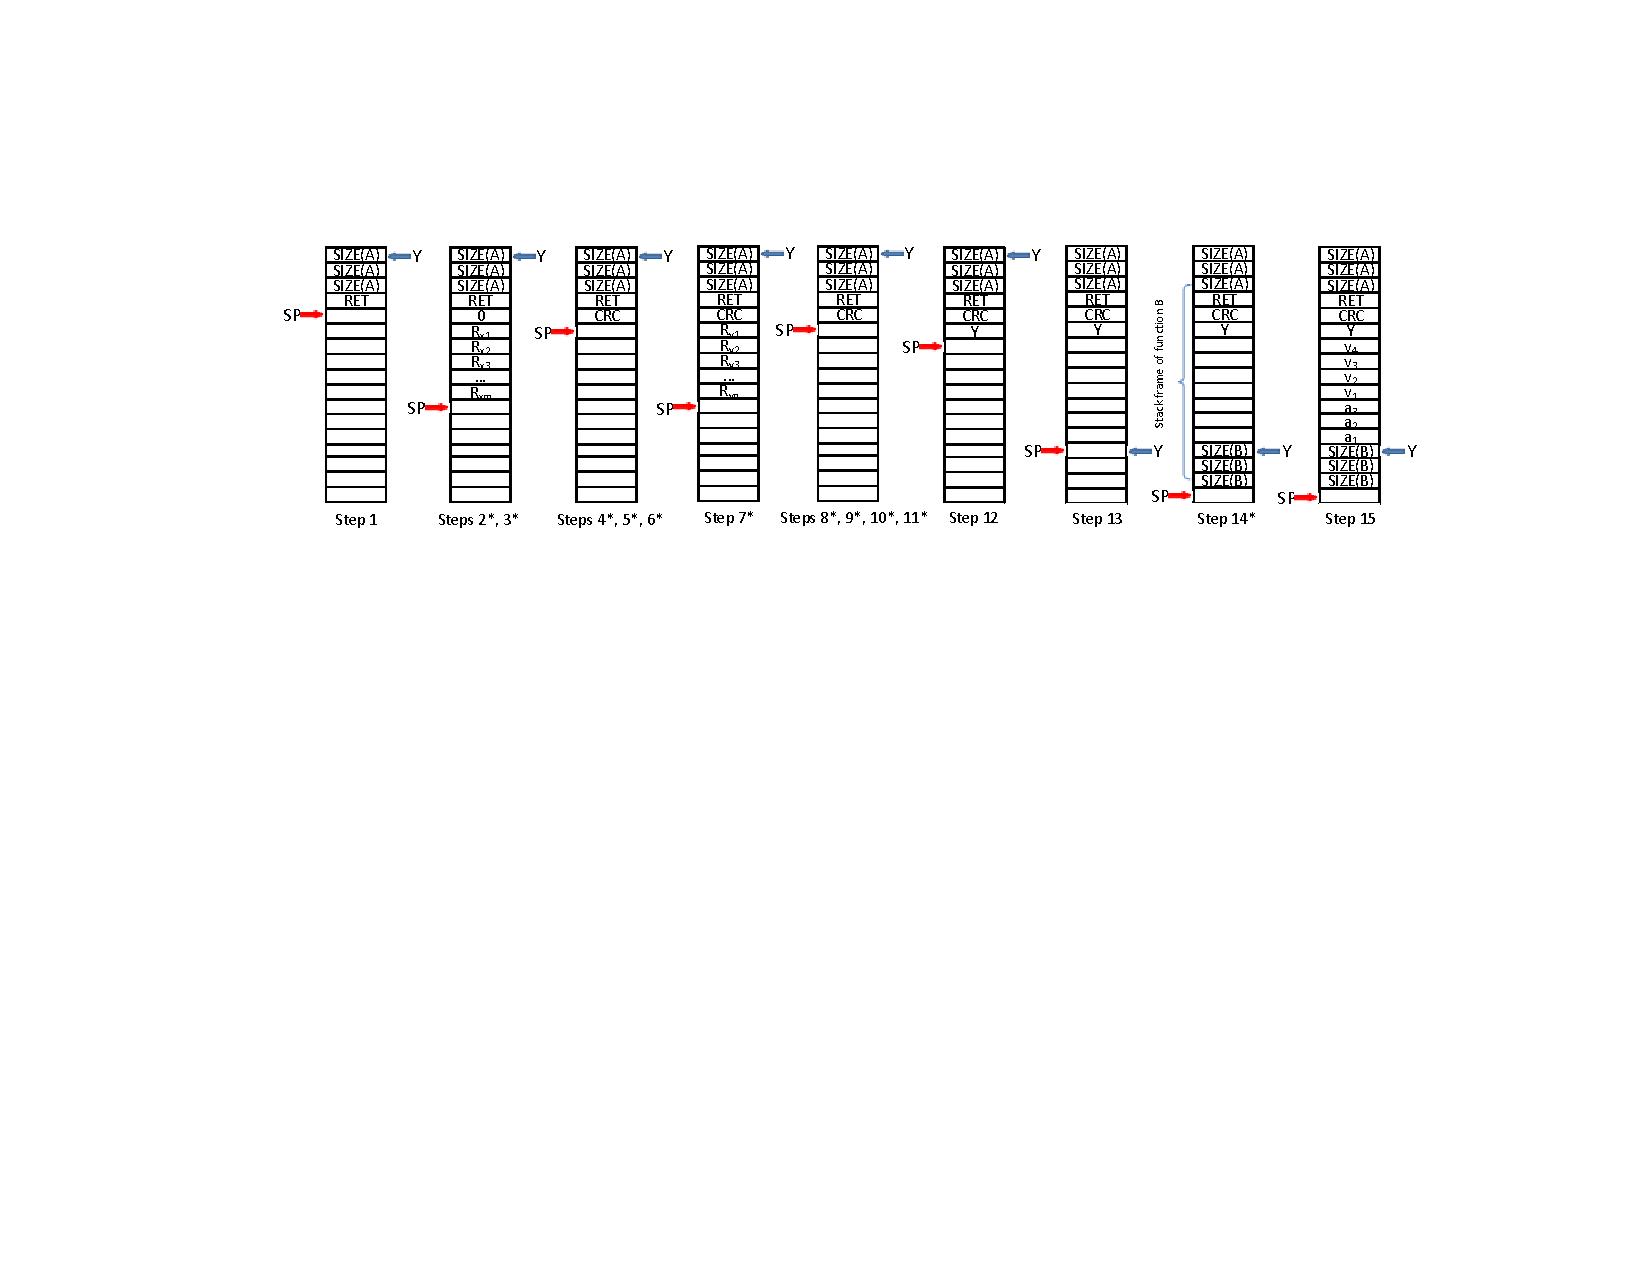
\includegraphics[width=1.0\textwidth]{figures/modified_function_operations_stack_pre_execution_v3}
	\vspace{-15pt}
	\caption{Modified Function Invocation Process}\label{fig:modified_function_operation_pre_execution}
\end{figure}
\vspace{-20pt}
The code segments injected at the beginning of each function are used to calculate a CRC over the caller's stack frame, and to save a duplicate of the caller's stack frame, as shown in Figure \ref{fig:modified_function_operation_pre_execution}. Each rectangle represents two stack bytes. The ``starred'' steps denote stack changes caused by the injected code. \texttt{SP} denotes the stack pointer, and \texttt{Y} denotes the stack frame pointer.

When a function \texttt{B} is called by a function \texttt{A}, the return address is pushed onto the stack automatically by the function call instruction (step 1). To calculate the CRC of the caller's stack frame, multiple registers are used, so they must be saved before the CRC calculation process and restored when the process is finished. To prevent the calculated CRC from being overwritten when the registers are restored, two bytes are pushed onto the stack as a placeholder (step 2) for the CRC result before the registers used to calculate the CRC are saved (step 3). After the CRC of function \texttt{A}'s stack frame is calculated (step 4), the CRC result is saved to the placeholder location (step 5). The registers used to calculate the CRC are then restored (step 6).

Next, the stack frame of the caller, function \texttt{A}, has to be saved. The registers used to save the frame are pushed (step 7). Next, the correct STP is selected by comparing the values of the three STP copies (step 8). Using the correct STP, the specified memory is then copied and saved in the SFS (step 9). After the STP copies are updated (step 10), the CRC registers are restored (step 11).

After the stack frame pointer of function \texttt{B} is saved (step 12), and the stack frame is established (step 13), three copies of the callee's frame size are pushed onto the stack (step 14), which is a key operation in the injected code. 

When a function is called, the callee does not have sufficient context regarding its caller, including the caller's stack frame address and size. It is impossible for a callee to calculate the CRC of it's caller's frame and to duplicate the frame without this information. To solve this problem, each function saves its frame size in the stack, which is used by its callee to perform the CRC calculation and frame copy. To ensure the correctness of the frame size, three copies are saved. Comparison is used to yield the correct value. 
\vspace{-10pt}
\subsubsection{Modified Function Return Process.}
The code segments injected at the end of each function are used to verify the stack frame of the caller, and to restore the stack frame if an SEU is detected, as shown in Figure \ref{fig:modified_function_operation_post_execution}. When function \texttt{B} returns, it first pops its stack frame size (step 1). After the space used to store the arguments and local variables is released (step 2), the stack frame pointer is restored (step 3). The CRC of function \texttt{A}'s stack frame is then calculated and temporarily stored in two registers (steps 4-6). The values stored in these registers are saved before the function return process. Next, the calculated CRC is compared with the CRC saved in the stack (step 7). If the two CRCs do not match, the saved stack frame of \texttt{A} is restored, and the STP is updated to release the space used to store the stack frame of \texttt{A} (steps 8-12). Again, the stack frame size of function \texttt{A} saved in the stack is used to support the CRC comparison and stack frame restoration (if needed). If the two CRCs match, the STP is updated (steps 13-14). After verification of \texttt{A}'s stack frame is complete, the CRC is popped from the stack (step 15). Finally, function \texttt{B} returns, and the return address is popped automatically (step 16).
\vspace{-20pt}
\begin{figure}
	\centering
	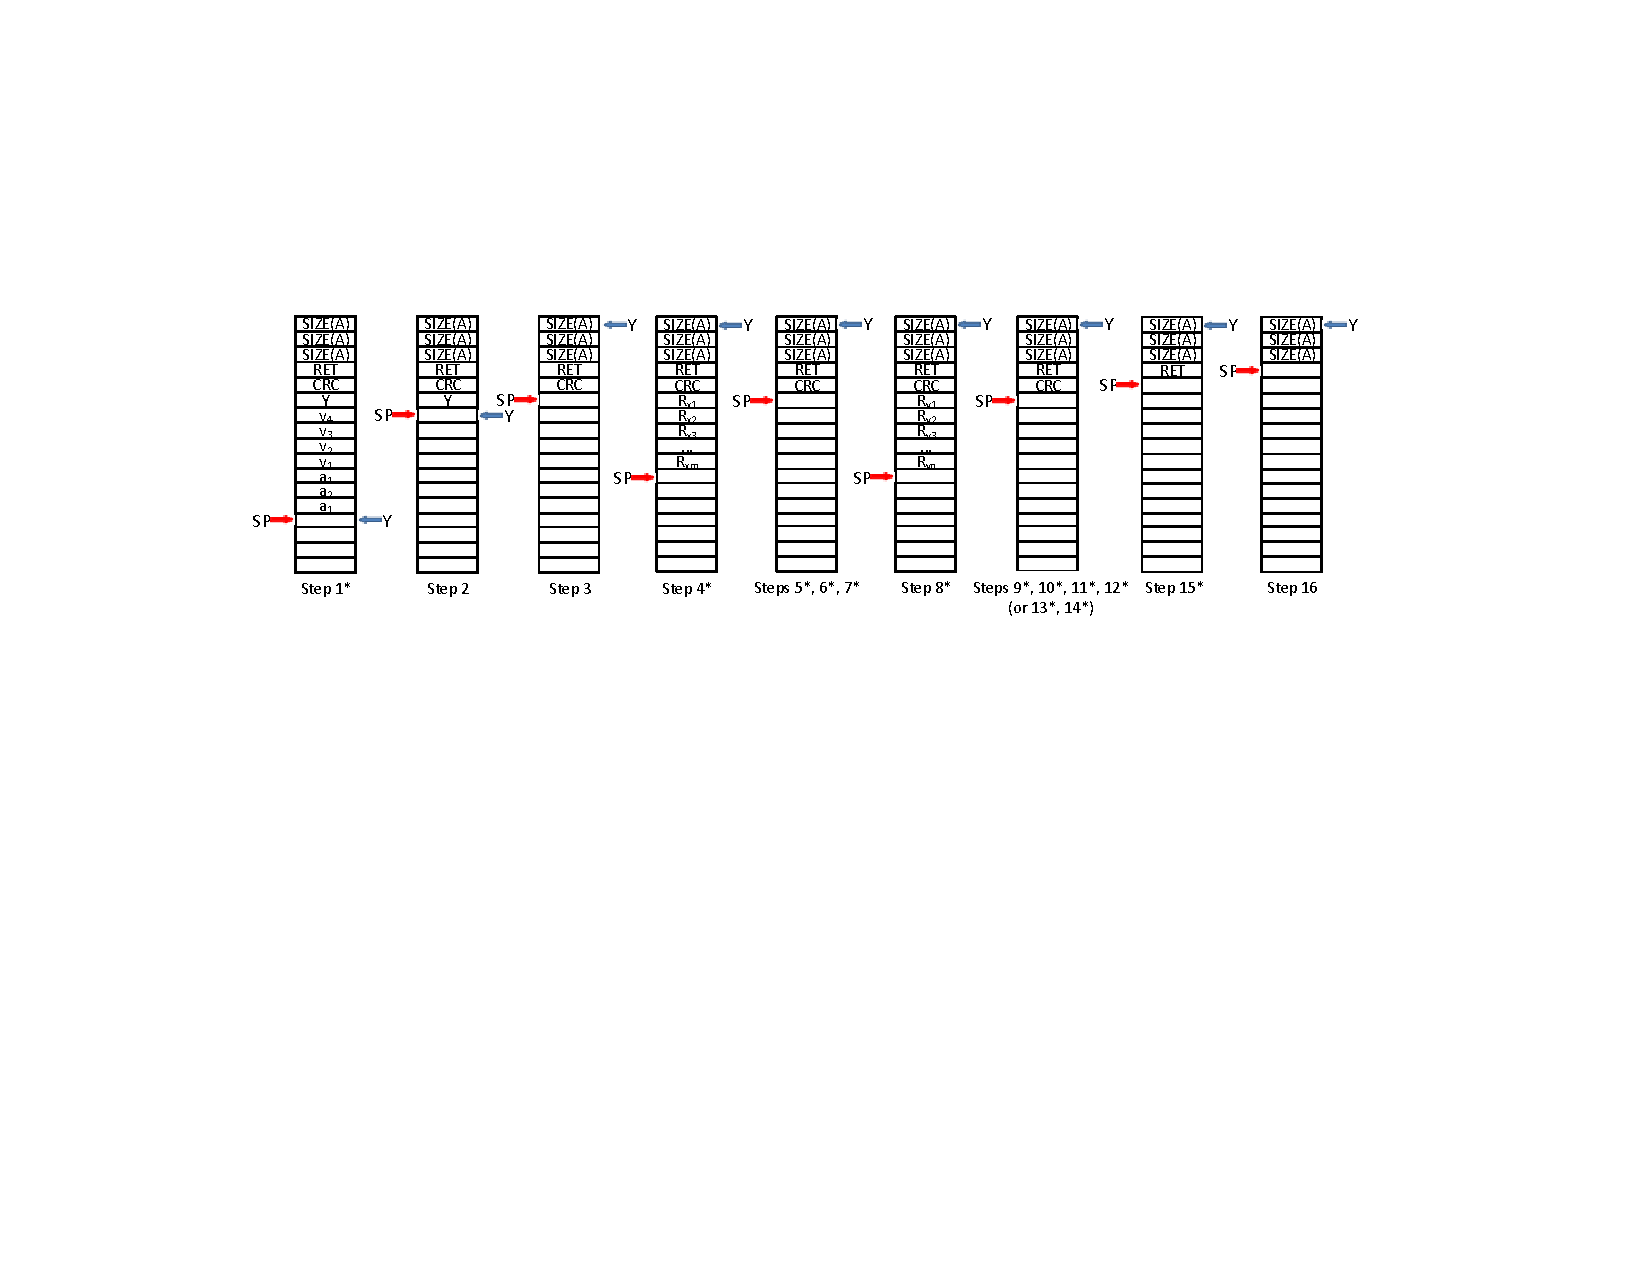
\includegraphics[width=1.0\textwidth]{figures/modified_function_operations_stack_post_execution_v3}
	\vspace{-20pt}
	\caption{Modified Function Return Process}\label{fig:modified_function_operation_post_execution}
\end{figure}
\vspace{-25pt}